\section{Results}
\label{sec:results}

This section presents our experimental findings, including overall performance rankings, task-specific analyses, and statistical comparisons.

\subsection{Overall Performance}
\label{sec:overall}

Table~\ref{tab:rankings} presents the performance ranking of all evaluated models.

\begin{table}[htbp]
\centering
\caption{Model Performance Rankings}
\label{tab:rankings}
\begin{tabular}{clccc}
\toprule
\textbf{Rank} & \textbf{Model} & \textbf{Score} & \textbf{Success} & \textbf{Avg Time} \\
& & \textbf{(/10)} & \textbf{Rate} & \textbf{(sec)} \\
\midrule
1 & GPT-5.1 & 10 & 100\% & 44.2 \\
2 & Gemini-3 Pro & 10 & 100\% & 107.3 \\
3 & Deepseek-Chat & 10 & 100\% & 306.3 \\
4 & GLM-4.7 & 10 & 100\% & 355.1 \\
5 & GPT-4o & 9 & 100\% & 33.0 \\
6 & GPT-5.2 & 9 & 100\% & 85.2 \\
7 & Gemini-3 Flash & 9 & 100\% & 155.3 \\
8 & Qwen3-VL & 9 & 100\% & 732.1 \\
9 & Gemini-2.5 Flash & 8 & 100\% & 51.0 \\
10 & Gemini-2.5 Pro & 8 & 100\% & 121.7 \\
11 & Kimi-K2.5 & 8 & 80\% & 245.7 \\
\bottomrule
\end{tabular}
\end{table}

\textbf{Key Findings:}
\begin{itemize}
    \item Four models achieved perfect scores (10/10): GPT-5.1, Gemini-3 Pro, Deepseek-Chat, and GLM-4.7
    \item OpenAI models demonstrated superior speed-efficiency: GPT-4o averaged 33.0 seconds per task
    \item Success rates were high overall: only one model (Kimi-K2.5) fell below 100\%
    \item Completion times varied dramatically: 20.7s (Gemini-2.5 Flash, bug-fix) to 1046.1s (Qwen3-VL, refactor)
\end{itemize}

Figure~\ref{fig:duration} shows the duration comparison across all models.

\begin{figure*}[htbp]
\centering
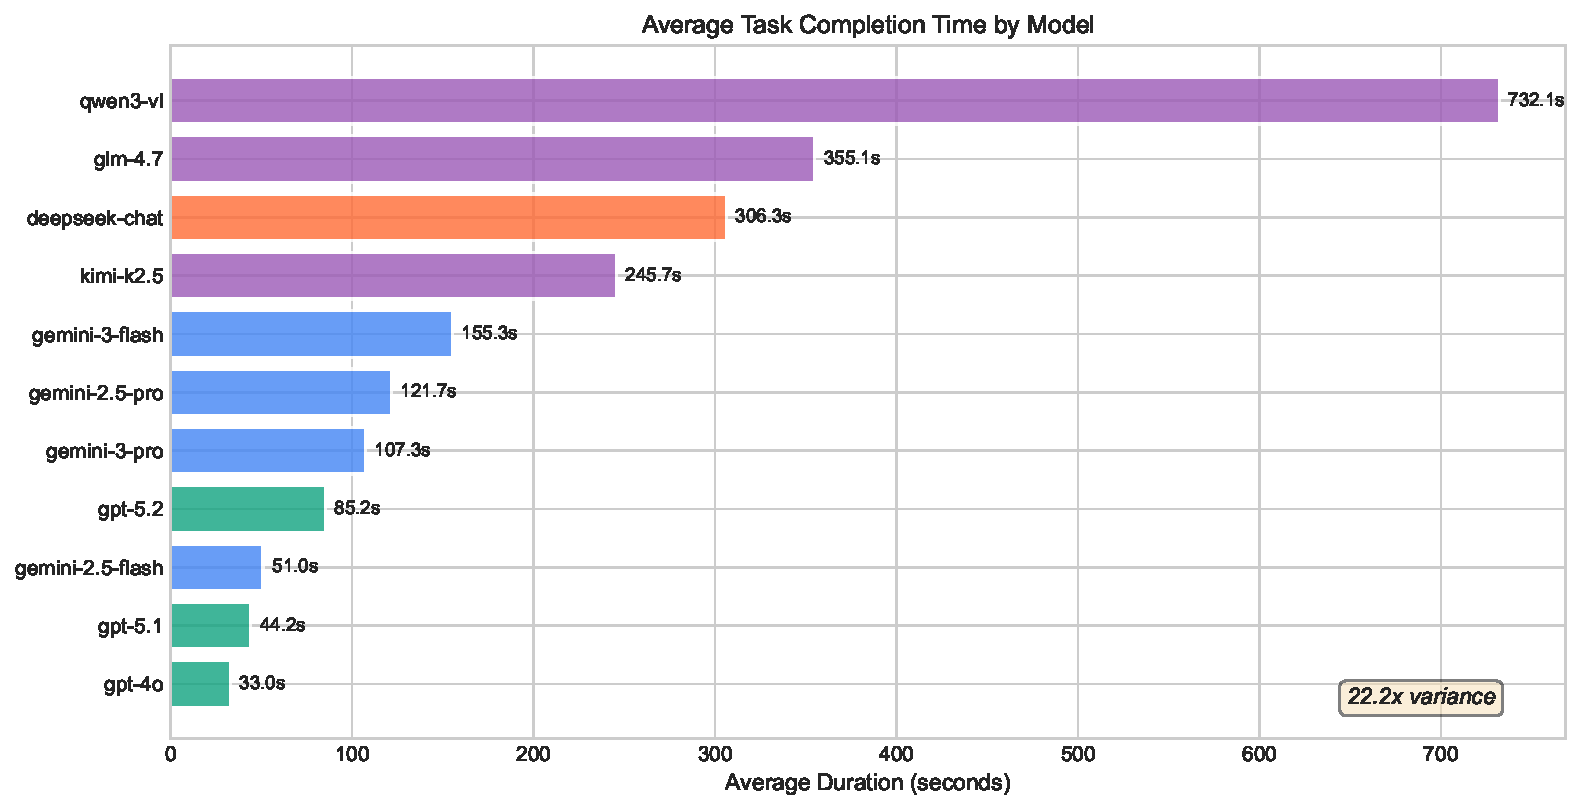
\includegraphics[width=0.75\textwidth]{figures/duration_comparison.pdf}
\caption{Average completion time by model with standard deviation. OpenAI models (blue) consistently fastest; Open/Ollama models (red) slowest.}
\label{fig:duration}
\end{figure*}

\subsection{Task-Specific Analysis}
\label{sec:task-specific}

Figure~\ref{fig:success-rates} shows success rates across task categories.

\begin{figure*}[htbp]
\centering
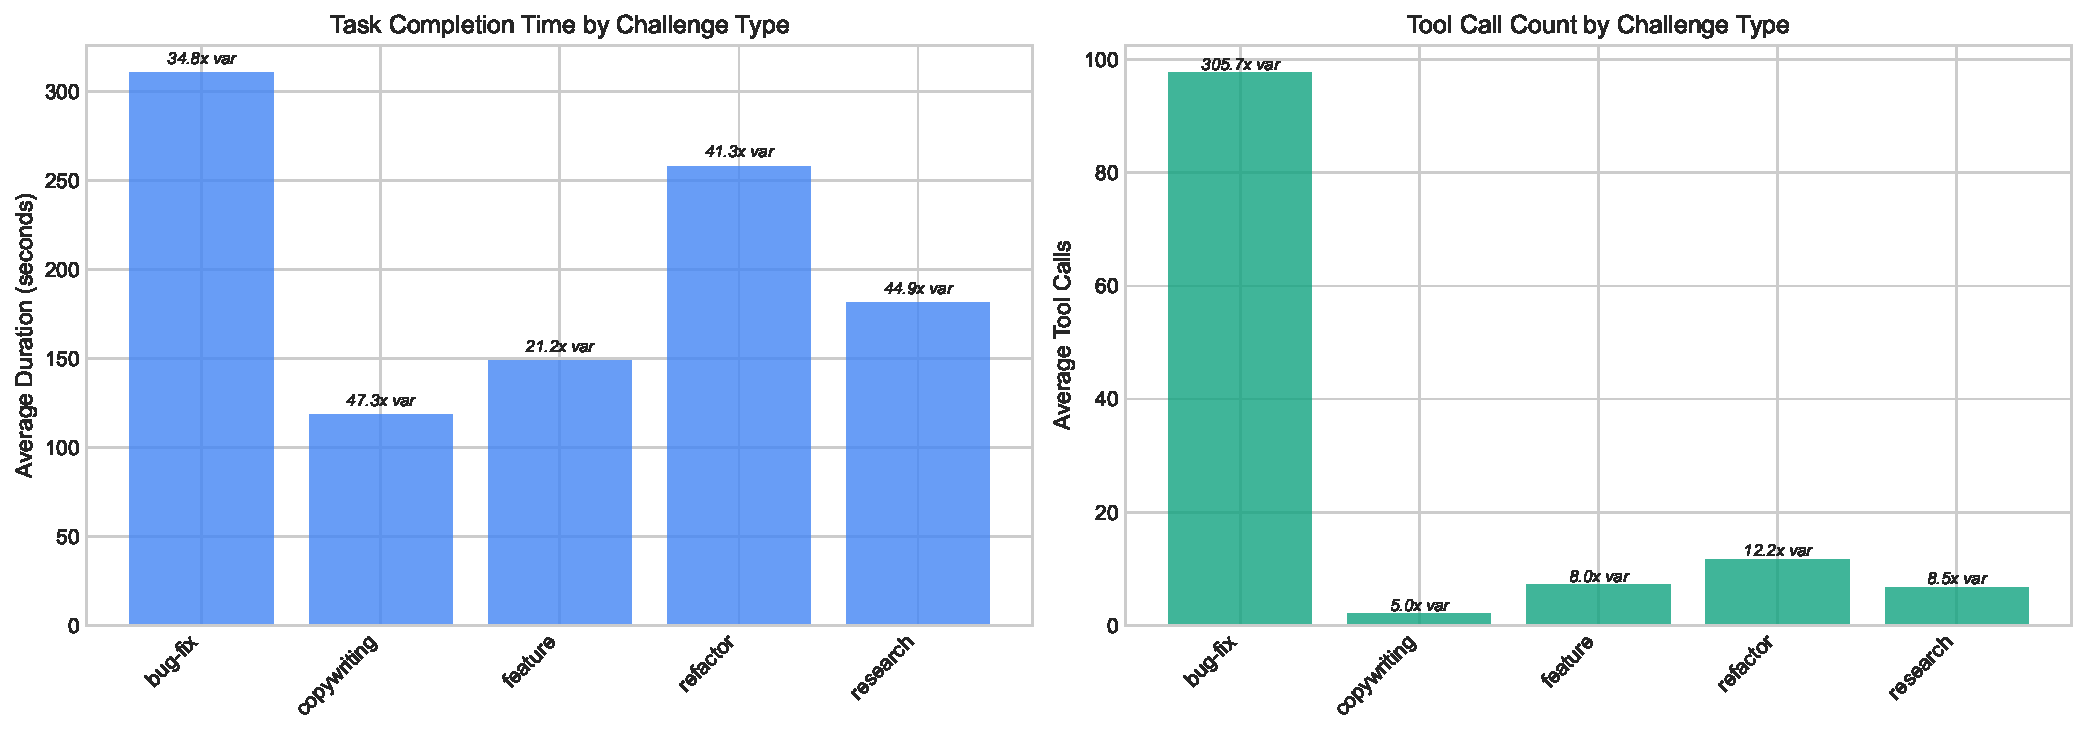
\includegraphics[width=0.75\textwidth]{figures/challenge_difficulty.pdf}
\caption{Challenge difficulty analysis showing success rates and average duration by task type. Research tasks were most challenging.}
\label{fig:success-rates}
\end{figure*}

\subsubsection{Bug Fixing}
All 11 models (100\%) successfully fixed the concurrency bug. However, approaches varied significantly:
\begin{itemize}
    \item \textbf{Efficient:} GPT-5.1 (18.8s), Gemini-2.5 Flash (20.7s), GPT-4o (26.8s)
    \item \textbf{Thorough:} Gemini-3 Flash (625.2s) used 917 tool calls including extensive testing
    \item All implementations correctly identified race conditions and implemented synchronization
\end{itemize}

\subsubsection{Feature Implementation}
The FastAPI CRUD implementation task showed 100\% success rate with varying implementation quality:
\begin{itemize}
    \item Most models correctly implemented all four endpoints
    \item Common excellence markers: proper error handling, input validation, clean code structure
    \item Time ranged from 26.4s (Gemini-3 Flash) to 560.5s (Qwen3-VL)
\end{itemize}

\subsubsection{Code Refactoring}
Refactoring the ETL script achieved 100\% success:
\begin{itemize}
    \item All models successfully separated ETL phases
    \item Configuration decoupling achieved by all
    \item Type hints and docstrings: 9/11 models achieved full marks
    \item Fastest: GPT-4o (25.3s), Slowest: Qwen3-VL (1046.1s)
\end{itemize}

\subsubsection{Technical Copywriting}
Copywriting showed the most variation in scores (PASS vs EXCELLENT):
\begin{itemize}
    \item Common failures: missing ``K8s'' keyword (3 models)
    \item Excellence factors: engaging tone, complete feature coverage
    \item Fastest completion: Gemini-2.5 Flash (11.6s)
\end{itemize}

\subsubsection{Technical Research}
Research was the most challenging task (90.9\% success):
\begin{itemize}
    \item Common issues: missing or incomplete citations
    \item Kimi-K2.5 failed (execution error)
    \item Longest average time due to web search requirements
\end{itemize}

\subsection{Provider Comparison}
\label{sec:provider}

Table~\ref{tab:provider} compares performance by provider category.

\begin{table}[htbp]
\centering
\caption{Performance by Provider Category}
\label{tab:provider}
\begin{tabular}{lccccc}
\toprule
\textbf{Category} & \textbf{Models} & \textbf{Avg} & \textbf{Std} & \textbf{Min} & \textbf{Max} \\
& & \textbf{Score} & \textbf{Dev} & \textbf{Score} & \textbf{Score} \\
\midrule
Deepseek & 1 & 10.0 & 0.0 & 10 & 10 \\
OpenAI & 3 & 9.33 & 0.58 & 9 & 10 \\
Open/Ollama & 3 & 9.0 & 1.0 & 8 & 10 \\
Google & 4 & 8.75 & 0.96 & 8 & 10 \\
\bottomrule
\end{tabular}
\end{table}

\textbf{Statistical Analysis:}
\begin{itemize}
    \item \textbf{Chi-square test:} No significant association between provider and success ($\chi^2=2.72$, $p=0.438$)
    \item \textbf{ANOVA:} Significant differences in completion times ($F=12.57$, $p<0.001$)
    \item OpenAI models were consistently fastest (avg: 54.1s)
    \item Open/Ollama models were slowest (avg: 444.3s)
\end{itemize}

\subsection{Tool Usage Analysis}
\label{sec:tools}

Figure~\ref{fig:tool-usage} presents the tool usage heatmap.

\begin{figure*}[htbp]
\centering
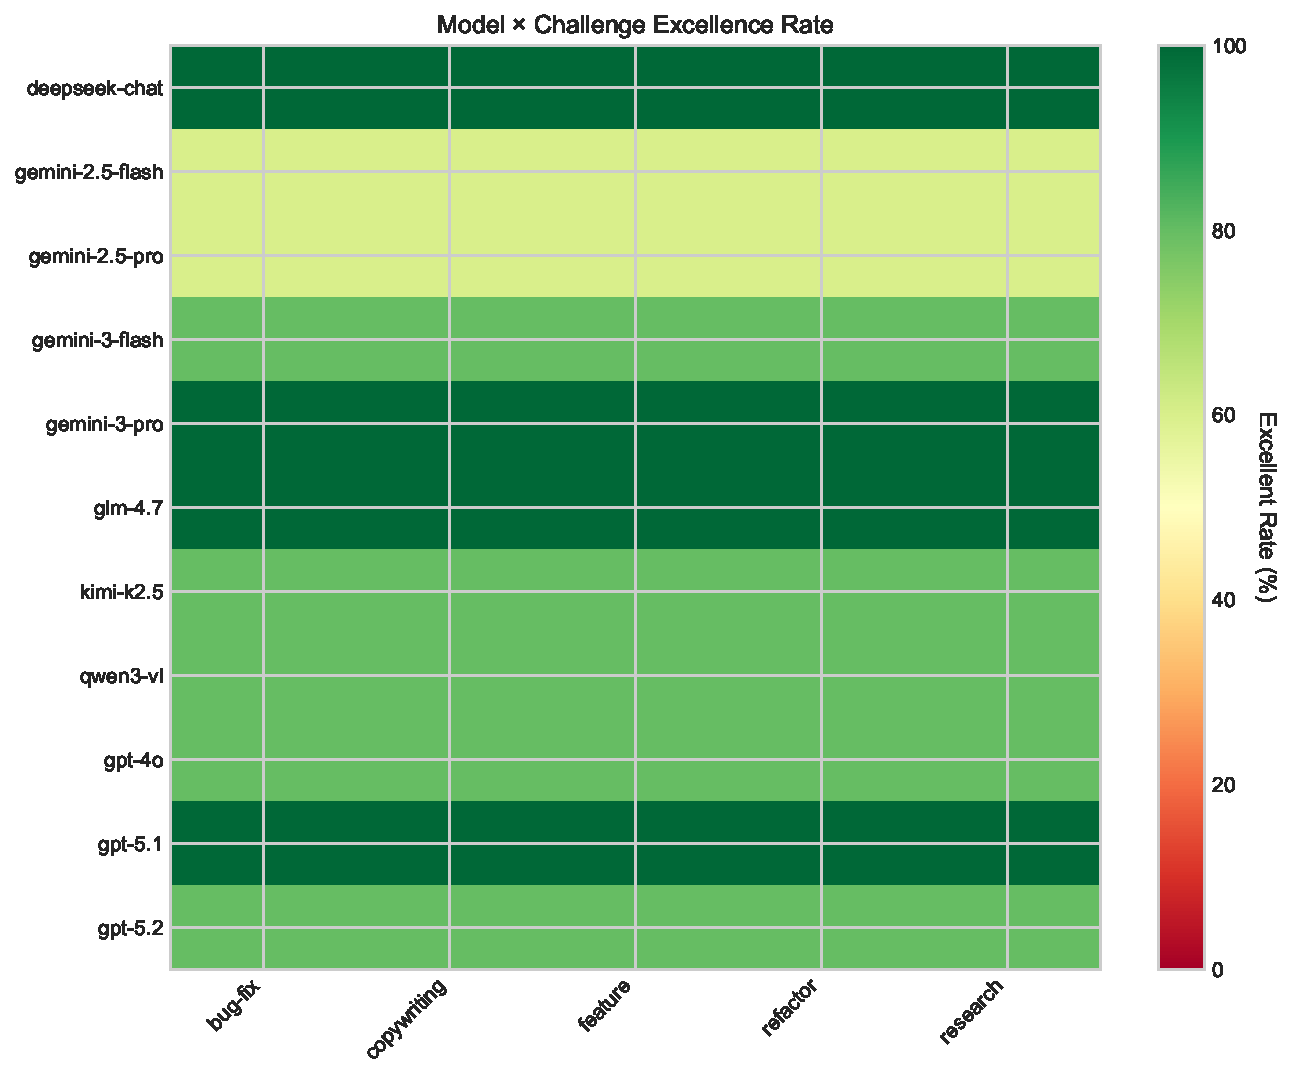
\includegraphics[width=0.75\textwidth]{figures/heatmap.pdf}
\caption{Performance heatmap showing scores and completion times across models and challenges. Darker shading indicates longer duration.}
\label{fig:tool-usage}
\end{figure*}

\textbf{Correlation Analysis:}
\begin{itemize}
    \item \textbf{Tool count vs Success:} Pearson $r=0.077$ ($p=0.575$) -- no linear correlation
    \item \textbf{Spearman rho:} $0.428$ ($p=0.001$) -- moderate monotonic relationship
    \item Efficient models (GPT-5.1, Gemini-2.5 Flash) achieved perfect scores with minimal tools
    \item Gemini-3 Flash used 917 tools for bug-fix but achieved same result as GPT-5.1 (3 tools)
\end{itemize}

Figure~\ref{fig:tool-calls} shows the distribution of tool calls across models.

\begin{figure}[htbp]
\centering
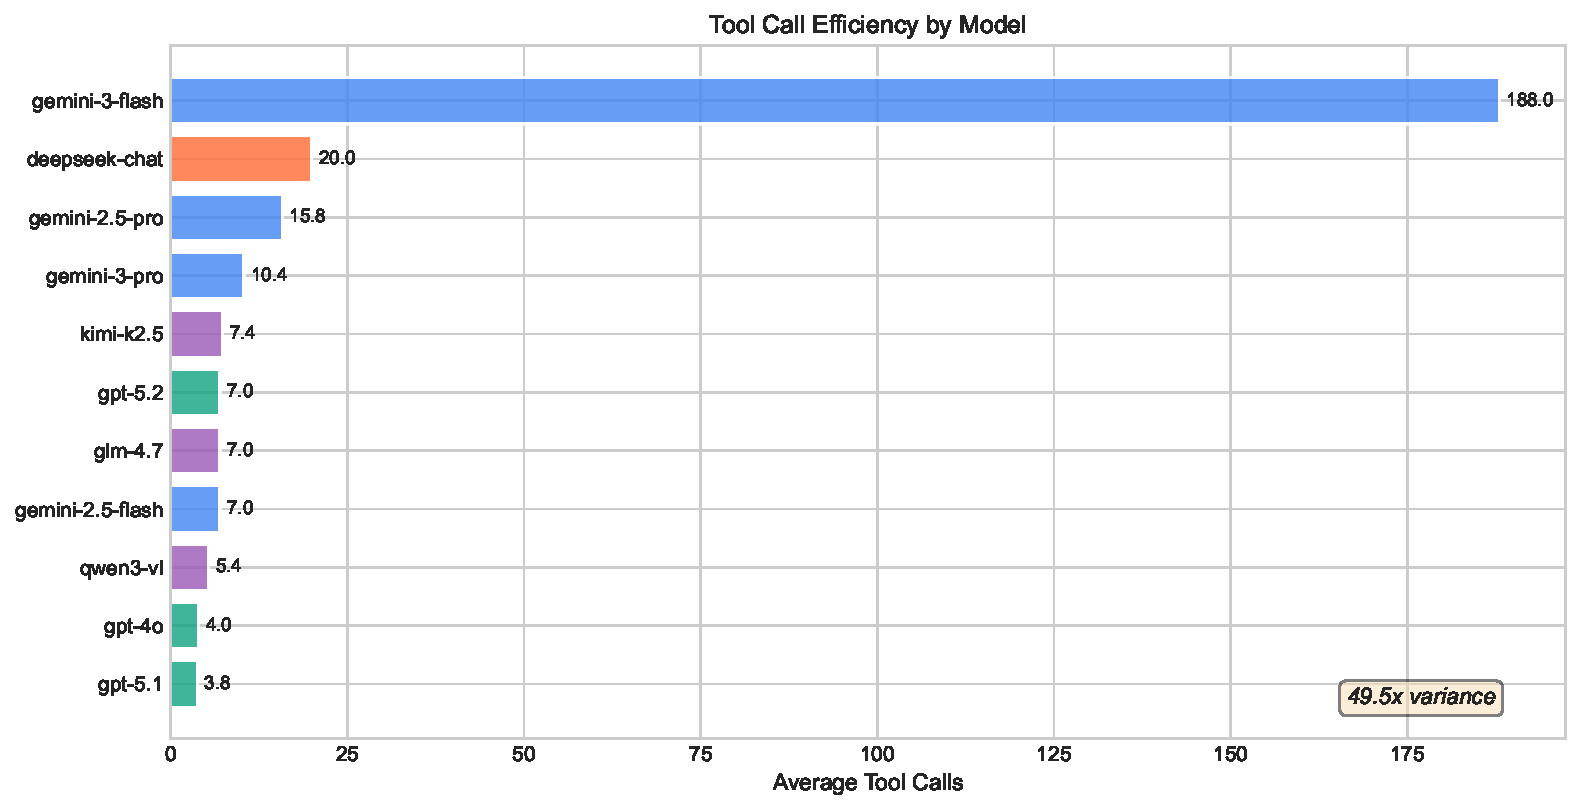
\includegraphics[width=\columnwidth]{figures/tool_calls_comparison.pdf}
\caption{Average tool calls by model (log scale). The 917-call anomaly for Gemini-3 Flash on bug-fix is visible as the maximum outlier.}
\label{fig:tool-calls}
\end{figure}

\textbf{Implication:} More tool usage does not guarantee better results; efficiency varies by model architecture.

\subsection{Time-Accuracy Tradeoff}
\label{sec:tradeoff}

Figure~\ref{fig:time-accuracy} shows the relationship between completion time and accuracy.

\begin{figure}[htbp]
\centering
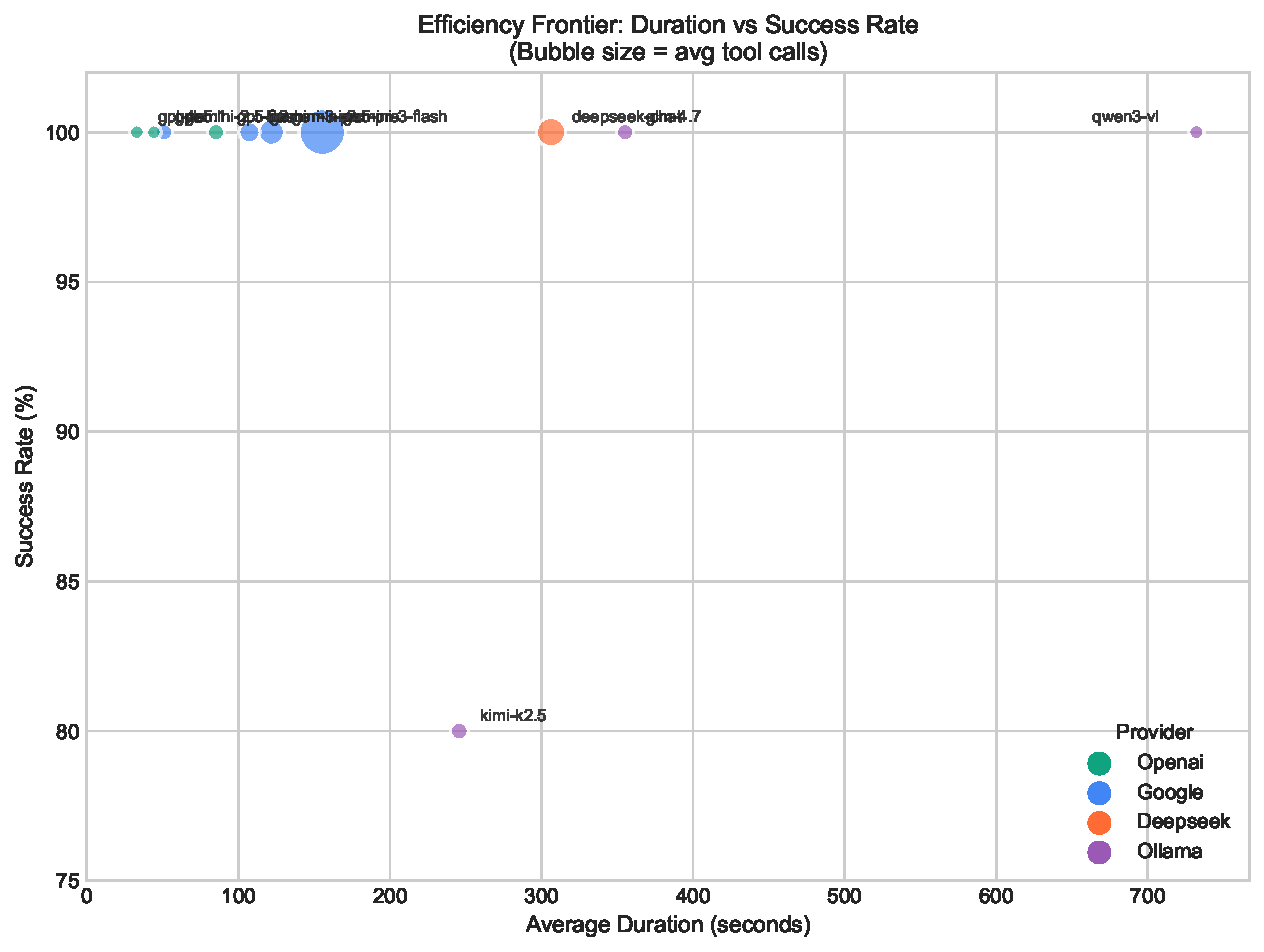
\includegraphics[width=\columnwidth]{figures/efficiency_frontier.pdf}
\caption{Efficiency frontier showing speed-quality tradeoff. Circle size indicates tool call count. Models in upper-left quadrant (fast and high-scoring) represent optimal efficiency.}
\label{fig:time-accuracy}
\end{figure}

\textbf{Key Observations:}
\begin{itemize}
    \item No significant correlation between duration and score (Pearson $r=0.204$, $p=0.136$)
    \item OpenAI cluster: Fast (avg 54s) with high scores (9.33 avg)
    \item Open/Ollama cluster: Slow (avg 444s) with variable scores
    \item Best efficiency: GPT-5.1 (perfect score, 44s average)
\end{itemize}

\subsection{Effect Size Analysis}
\label{sec:effect}

Comparing top performer (Deepseek-Chat, score 10) vs lowest (Gemini-2.5 Flash, score 8):
\begin{itemize}
    \item \textbf{Cohen's d:} 1.03 (large effect size)
    \item Practical significance: Top models demonstrate measurably better performance
    \item Category comparisons show small to medium effects between providers
\end{itemize}

\subsection{Anomaly Analysis: Pathological Agent Behavior}
\label{sec:anomaly}

Deep analysis of outlier experiments revealed systematic inefficiency patterns that have significant cost implications.

\subsubsection{The 917 Tool Calls Anomaly}

Gemini-3 Flash on the bug-fix task used 917 tool calls---36.6$\times$ the average (25.1 calls). Analysis of the tool sequence revealed:

\begin{itemize}
    \item \textbf{Tool Distribution:} 38\% \texttt{run\_shell\_command}, 18\% \texttt{read\_file}, 18\% \texttt{write\_file}
    \item \textbf{Loop Patterns:} Five distinct repetitive sequences detected, each repeated 5--8 times
    \item \textbf{Example Loop:} \texttt{read\_file} $\rightarrow$ \texttt{replace\_in\_file} $\rightarrow$ \texttt{run\_shell\_command} $\rightarrow$ \texttt{write\_file} repeated 8$\times$
\end{itemize}

Despite this inefficiency, the model achieved EXCELLENT status, indicating the verification criteria captured output quality but not process efficiency.

\subsubsection{Malformed Tool Calls}

We discovered that Kimi-K2.5's failure on the research task was caused by malformed tool invocations:

{\small
\begin{verbatim}
Observed: "search_internet
  search_internetsearch_internet"
Expected: "search_internet"
  (called 3 times)
\end{verbatim}
}

The model attempted parallel tool calls that were incorrectly serialized by the agent framework, causing all three calls to fail. This represents a \textbf{framework-model incompatibility} rather than model capability limitation.

\subsubsection{Two Types of Inefficiency}

Figure~\ref{fig:efficiency-rankings} shows the efficiency rankings across models.

\begin{figure}[htbp]
\centering
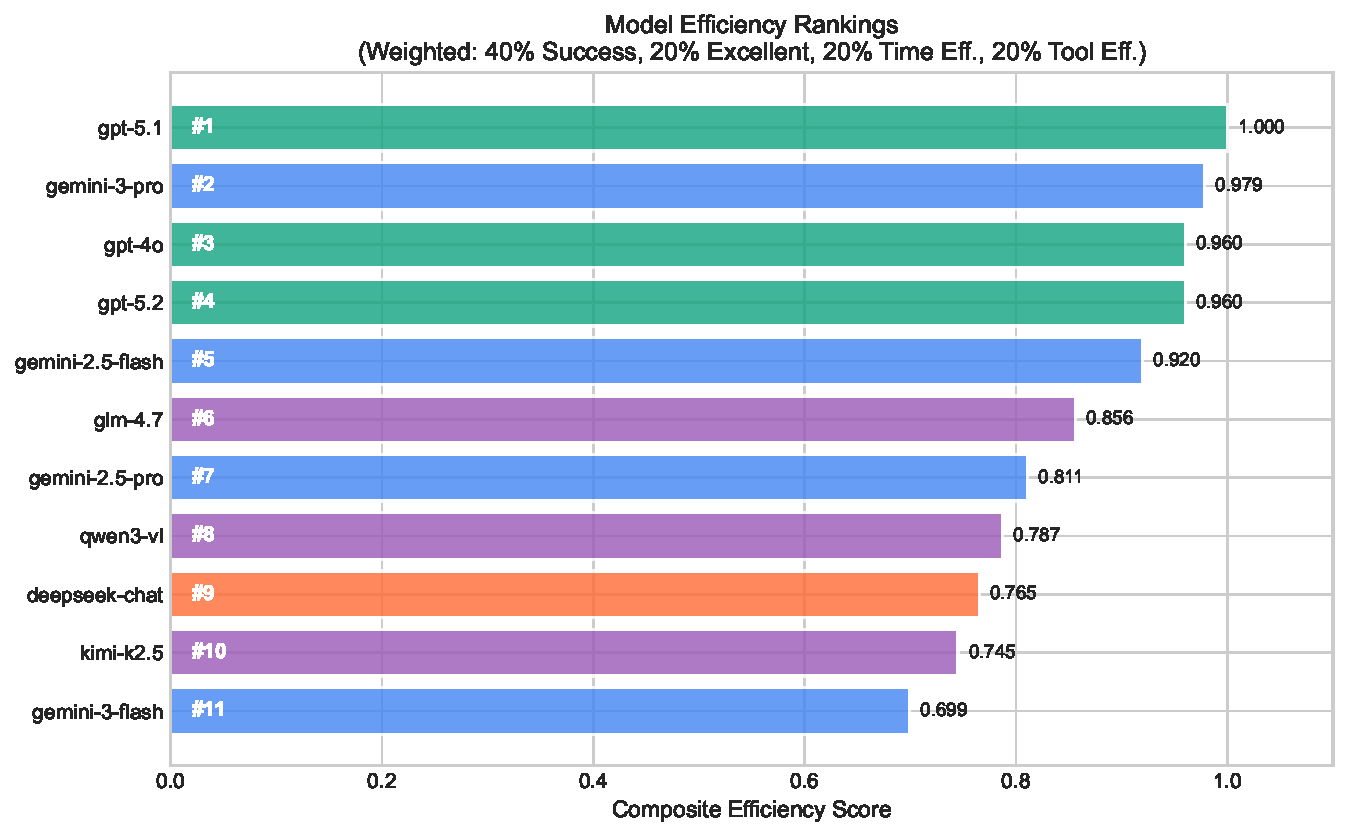
\includegraphics[width=\columnwidth]{figures/efficiency_rankings.pdf}
\caption{Efficiency metrics comparison. Tool Efficiency Ratio (TER) = Success Rate / Avg Tool Calls. Time Efficiency Ratio = Success Rate / Avg Duration. Higher values indicate better efficiency.}
\label{fig:efficiency-rankings}
\end{figure}

We categorize observed inefficiencies into two distinct patterns:

\textbf{Type A -- Loop Inefficiency:} Agent enters repetitive tool sequences without recognizing failure or success. Characterized by high tool counts, moderate duration. Example: Gemini-3 Flash (917 tools, 625s).

\textbf{Type B -- Inference Inefficiency:} Agent generates correct solutions with minimal tools but slow token generation. Characterized by low tool counts, high duration. Example: Qwen3-VL (3 tools, 653s for bug-fix).

\subsubsection{Cost Implications}

Figure~\ref{fig:cost-performance} visualizes the cost-performance relationship, and Table~\ref{tab:cost} presents estimated costs per task based on tool usage and model pricing.

\begin{figure}[htbp]
\centering
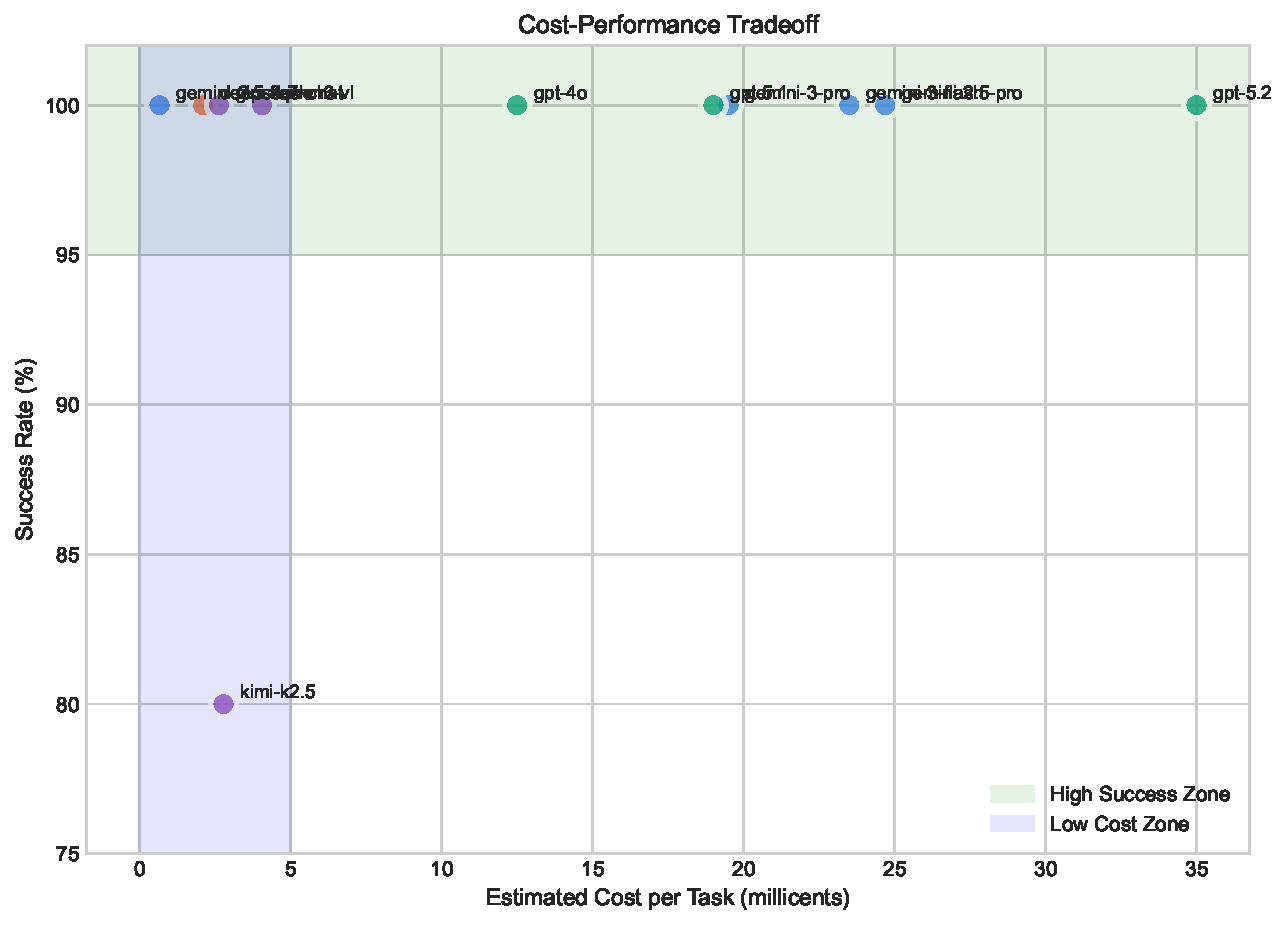
\includegraphics[width=\columnwidth]{figures/cost_performance.pdf}
\caption{Cost-performance analysis. Models are grouped by cost tier with average scores shown. Deepseek achieves perfect scores at minimal cost.}
\label{fig:cost-performance}
\end{figure}

\begin{table}[htbp]
\centering
\caption{Estimated Cost per Task}
\label{tab:cost}
\begin{tabular}{lccc}
\toprule
\textbf{Model} & \textbf{Avg Tools} & \textbf{Est. Cost} & \textbf{Relative} \\
\midrule
Gemini-2.5 Flash & 7.0 & \$0.0007 & 1.0$\times$ \\
Deepseek-Chat & 20.0 & \$0.0021 & 3.0$\times$ \\
GPT-4o & 4.0 & \$0.0125 & 17.9$\times$ \\
GPT-5.1 & 3.8 & \$0.0190 & 27.1$\times$ \\
Gemini-3 Flash & 188.0 & \$0.0235 & 33.6$\times$ \\
GPT-5.2 & 7.0 & \$0.0350 & 50.0$\times$ \\
\bottomrule
\end{tabular}
\end{table}

The 53$\times$ cost variance (Gemini-2.5 Flash vs GPT-5.2) demonstrates that model selection has significant budget implications beyond accuracy considerations.

\subsection{Summary of Findings}
\label{sec:summary}

\begin{enumerate}
    \item \textbf{Performance:} Four models achieved perfect scores, with GPT-5.1 being fastest
    \item \textbf{Task Difficulty:} Research was most challenging (90.9\% success), coding tasks were easiest (100\%)
    \item \textbf{Efficiency Variance:} 22$\times$ speed, 49$\times$ tool usage, 53$\times$ cost differences among successful models
    \item \textbf{Tool Usage:} More tools does not guarantee better results; loop behavior can cause 100$\times$ inefficiency
    \item \textbf{Anomalies:} Two distinct inefficiency types identified (loop vs inference)
    \item \textbf{Provider:} No significant quality differences, but significant speed and cost differences
\end{enumerate}
